\documentclass[a4paper,dvips,12pt]{article}
%%%%%%%%%%%%%%%%%%%%%%%%%%%%%%%%%%%%%%%%%%%%%%%%%%%%%%%%%%%%%%%%%%%%%%%%%%%%%%%%%%%%%%%%%%%%%%%%%%%%%%%%%%%%%%%%%%%%%%%%%%%%%%%%%%%%%%%%%%%%%%%%%%%%%%%%%%%%%%%%%%%%%%%%%%%%%%%%%%%%%%%%%%%%%%%%%%%%%%%%%%%%%%%%%%%%%%%%%%%%%%%%%%%%%%%%%%%%%%%%%%%%%%%%%%%%
\usepackage{url}
\usepackage{setspace}
\usepackage{fullpage}
\usepackage{caption}
\usepackage{amssymb}
\usepackage{amsmath}
\usepackage{amsfonts}
\usepackage{longtable}
\usepackage{rotfloat}
\usepackage{rotating}
\usepackage{tabularx}
\usepackage{booktabs}
\usepackage{afterpage}
\usepackage{graphicx}
\usepackage{harvard}
\usepackage{ucs}
\usepackage[T1]{fontenc}
\usepackage{lmodern}


\setcounter{MaxMatrixCols}{10}
%TCIDATA{OutputFilter=Latex.dll}
%TCIDATA{Version=5.50.0.2960}
%TCIDATA{<META NAME="SaveForMode" CONTENT="1">}
%TCIDATA{BibliographyScheme=BibTeX}
%TCIDATA{LastRevised=Wednesday, May 01, 2013 22:05:19}
%TCIDATA{<META NAME="GraphicsSave" CONTENT="32">}

\newtheorem{theorem}{Theorem}
\newtheorem{acknowledgement}[theorem]{Acknowledgement}
\newtheorem{algorithm}[theorem]{Algorithm}
\newtheorem{axiom}{Assumption}
\newtheorem{case}[theorem]{Case}
\newtheorem{claim}[theorem]{Claim}
\newtheorem{conclusion}[theorem]{Conclusion}
\newtheorem{condition}[theorem]{Condition}
\newtheorem{conjecture}[theorem]{Conjecture}
\newtheorem{corollary}{Corollary}
\newtheorem{criterion}[theorem]{Criterion}
\newtheorem{definition}{Definition}
\newtheorem{example}[theorem]{Example}
\newtheorem{exercise}[theorem]{Exercise}
\newtheorem{lemma}{Lemma}
\newtheorem{notation}[theorem]{Notation}
\newtheorem{problem}[theorem]{Problem}
\newtheorem{proposition}{Proposition}
\newtheorem{remark}{Remark}
\newtheorem{solution}[theorem]{Solution}
\newtheorem{summary}[theorem]{Summary}
\newenvironment{proof}[1][Proof]{\textbf{#1.} }{\ \rule{0.5em}{0.5em}}
\renewcommand{\baselinestretch}{1.5}
\newcommand{\eps}{\varepsilon}
\hyphenation{sub-si-di-zing}
\begin{document}

\begin{center}
{\Large
Appendix to ``Education and Crime over the Life Cycle''}
\bigskip

Giulio Fella and Giovanni Gallipoli
\end{center}
\setcounter{section}{0}
\setcounter{page}{1}
\setcounter{equation}{0}
\setcounter{figure}{0}
\setcounter{table}{0}
\bigskip

\section{Appendix: Stationary Equilibrium}
\label{sec:stat-equil}
% The equilibrium concept we use is that of recursive, stationary,
% competitive equilibrium following \citeasnoun{Stokey-Lucas-Prescott-89}. While
% the concept is standard in the literature, the dimension of the state
% space and the degree of life cycle heterogeneity in the present model
% are such that a formal definition of equilibrium is very heavy on
% notation. For this reason, we relegate it to Appendix A.

Let $z_{j}^{x}\in Z^{x}_{j}$ denote the state implicit in the recursive
representation of the problem for an individual of age $j$ and type $x,$
where $x$ can take value $s$ (student), $n$ (worker out of jail) and $p$
(worker in jail).

For a given set of government policies $\left\{pen,G,sub^{e},t_{l},t_{k}%
\right\}, $ tuition fees $tuit^e$ and apprehension probability $\pi_{p}$, a \emph{%
  stationary recursive equilibrium} is a collection of (i) policy functions
for consumption $c^{x}_{j}(z^{x}_{j})$, saving $%
a^{x}_{j+1} (z^{x}_{j}),$ bequests $b,$ education $%
\{i^{s}_{H}(z^{s}_{0}),i^{s}_{C}(z^{s}_{j_H})\}$ and crime $%
\{\tau^{n}_{j}(z^n_j)\};$ (ii) value functions $\{V^{x}_{j}(z^{x}_{j})\};$
decision rules \linebreak $\left\{ K,H_{L},H_{H},H_{C}\right\} $ for firms; (iv) prices
$\left\{ r,w^{L},w^{H},w^{C}\right\}; $ (v) a victimization rate $%
\pi_{\upsilon};$ (vi) an average labor income $\overline{wh};$ (vii)
time-invariant measures $\{\mu^{s}_{j},\mu^{n}_{j},\}$ and $\Gamma(a)$ that
satisfy the following conditions.

\begin{enumerate}
\item Given prices$\left\{ r,w^{L},w^{H},w^{C}\right\}:$

\begin{itemize}
\item for $x=s,n$ the decision rules \{$%
c^{x}_{j}(z^{x}_{j}),a^{x}_{j+1}(z^{x}_{j}) $\} and the value functions $%
V^{x}_{j}(z^{x}_{j})$ solve respectively equations (13)-(15) for $x=s$, equation (16) for $x=n$ and $j<j_{r},j\neq
j_{b},$ equation (18) for $x=n$ and $j=j_{b},$ equation (19)
for $j\geq j_{r};$

\item the decision rule $a^{p}_{j+1}(z^{x}_{j})$ satisfies equation (11)
  with $i^p=1$ and the associated value function $%
  V^{p}_{j}(z^{p}_{j})$ solves equation (17);

\item the decision rule $b$ solves equation (18);

\item the education decisions $\{i^{s}_{L}(z^{s}_{0}),i^{s}_{H}(z^{s}_{j_H})%
\}$ solve equations (12) and (15);

\item the crime decision $\tau_{j}(z^{n}_{j})$ solves equation (16).
\end{itemize}

\item Given prices$\left\{ r,w^{L},w^{H},w^{C}\right\},$ input demands $%
\left\{ K,H_{L},H_{H},H_{C}\right\} $ maximize profits for the
representative firm
\begin{equation*}
r=(1-t_{k})(F_{K}-\delta)  \label{fock}
\end{equation*}
and
\begin{equation*}
w^{e} =(1-t_{l})F_{H_{e}},\ \text{for } e\in \{L,H,C\}.
\end{equation*}

\item The asset market clears
\begin{equation*}
K=\sum_{j,x} \int \limits_{Z^{x}_{j}}a^{x}_{j+1}(z^{x}_{j})d\mu^{x}_{j}.
\end{equation*}%


\item The labor markets for each educational level clear\footnote{%
By Walras law, market clearing on all factor markets ensures that the goods
market clears.}
\begin{equation*}
H_{e}=\sum_{j<j_{r}}\int \limits_{\{z^{n}_{j}:e=i\}}h_{j}\left(
\theta,e\right)\left[1-\pi_{p}\tau(z^{n}_{j})-\pi_{p} f \tau(z^{n}_{j-1})\right] d\mu^{n}_{j},\ \text{for } i\in
\{0,1,2\}.
\end{equation*}
where the supply of labor on the right hand side of the above equation
is made up only of individuals out of jail. In the calibrated model the
prison term is strictly between one and two years. It follows that in
the stationary equilibrium, the number of
convicted felons in each age group $j$ is the fraction
$(1-\pi_{p}\tau(z^{n}_{j})-\pi_{p}f\tau(z^{n}_{j-1}))$ of workers that
have not been arrested at age $j$ or that, if arrested at age $j-1$, have not been released. To clarify notation, the argument $z^{n}_{j-1}$ in the equation above is meant as a function of $z^{n}_{j}$ such that $z^{n}_{j-1}$ is identical to $z^{n}_{j}$ with the only exception that asset holdings at age $j$ satisfy $a_{j}=a^{p}_{j-1}(z^{n}_{j-1})$.

\item The government budget is balanced
\begin{equation*}
G+E+PRIS+PENS =\frac{t_{k}}{1-t_{k}}rK+\frac{t_{l}}{1-t_{l}}\sum_{e} w^{e}H_{e}.
\end{equation*}
Total government outlays on the left hand side of the above equation are the
sum of exogenous wasteful expenditure $G,$ education subsidies $%
E=\sum_{j,i}\int_{\{z^{s}_{j}:e=i\}} sub^{i} \thinspace d\mu^{s}_{j},$ for $%
i=\{L,H,C\},$ aggregate prison expenditure\footnote{%
In stationary equilibrium, the number of convicted felons in each age group
equals a fraction $\pi_{p}\tau(z^{n}_{j}))$ of the corresponding number of
workers.} $PRIS=\sum_{j<j_{r}}\int _{Z^{n}_{j}}m \thinspace
\pi_{p}\tau(z^{n}_{j})) d\mu^{n}_{j}$ and aggregate pension expenditure $%
PENS=\sum_{j\geq j_{r}}\int_{Z^{n}_{j}}pen\thinspace d\mu^{n}_{j}.$

\item The victimization rate coincides with the crime rate
\begin{equation*}
\pi_{\upsilon}=\left(\sum_{j<j_{r}} \int_{
Z^{n}_{j}}(1-\pi_{p}\tau(z^{n}_{j})-\pi_{p}f\tau(z^{n}_{j-1})) d\mu^{n}_{j} \right)
^{-1}\sum_{j<j_{r}}\int_{Z^{n}_{j}}\tau_{j}(z^{n}_{j}) d\mu^{n}_{j},
\end{equation*}
and equals the total number of crimes divided by the total number of workers
out of jail.

\item The average disposable labor income satisfies
\begin{equation*}
\overline{wh}=\left(\sum_{j<j_{r}}
\int_{Z^{n}_{j}}(1-\pi_{p}\tau(z^{n}_{j})-\pi_{p}f\tau(z^{n}_{j-1})) d\mu^{n}_{j} \right) ^{-1}
\sum_{e}w^{e}H_{e}.
\end{equation*}

\item The distribution of wealth at birth $\Gamma(a_{0})$ equals the
distribution of bequests
\begin{equation*}
\Gamma(a_{0})=\int_{\{z^{n}_{j_{b}}:b(z^{n}_{j_{b}})\leq
a_{0}\}}d\mu^{n}_{j_{b}}. %+\mathbb{I}_{a_{0}=0}\tau_{j_{b}}(z^{n}_{j_{b}})\mu^{n}_{j_{b}}
\end{equation*}

\item The vector of measures $\mu=\{\mu^{s}_{0},...,\mu^{s}_{\bar
j};\mu^{n}_{0},...,\mu^{n}_{\bar j}\}$ is the fixed point of $%
\mu(Z)=Q(Z,\mu) $ where $Z$ is the generic subset of the Borel sigma algebra
$\mathfrak{B}_{Z}$ defined over the state space $\mathbb{Z}=\prod_{j,x}
Z^{x}_{j},$ the Cartesian product of all $Z^{x}_{j}.$ The mapping $Q(Z,\mu)$
is the transition function associated with the individual decisions, the law
of motion for the shocks $\{\chi,\theta,v,i^{p},\varepsilon^{e}_{j}\}$ and
the survival probabilities $\{\lambda_{j}\}.$
\end{enumerate}

\section{Appendix: Computation and calibration}

\label{sec:computation}

Let $Z=\{\xi,\nu_{1},\nu_{2},\nu_{3},\underline a,\underline
\chi,\alpha,\beta,\rho_{\theta \chi},\kappa,\bar c\}$ denote the set of
calibrated parameters other than the utility cost of studying parameters $%
\{\psi^{H}(\theta),\psi^{C}(\theta)\}$. Given a guess for $Z$, $%
\{\psi^{H}(\theta),\psi^{C}(\theta)\}$ and the vector of equilibrium prices $%
\{r,w^{L},w^{H},w^{C}\}$ we calibrate the model in the following way.

\begin{enumerate}
\item We solve for the consumer decisions rules and value function and the
representative firm factor demand functions.

\item We simulate the model up to the age of the college choice and solve
for the values of $\{\psi^{H}(\theta),\psi^{C}(\theta)\}$ that match the
enrolment rates in the data. Using the new values as our new guess, we
simulate again the economy up to the age of college choice and iterate on
this procedure until the values of $\{\psi^{H}(\theta),\psi^{C}(\theta)\}$
converge.

\item We simulate the model at the remaining ages and compute the aggregate
factor supplies. We compare the marginal products of the four factors to
our guess for their prices. If the two differ by more than the specified
tolerance, we adjust the guess for prices and solve again the problem,
starting from point 1. until convergence (market clearing).

\item When factor prices have converged, we evaluate the loss function --
the sum of squared deviations of the model from the data calibration moments
-- at the simulated model moments. We use a multi-dimensional optimization
method to update the guess on $Z$ and continue to iterate starting from
point 1. above until convergence.
\end{enumerate}

Concerning point 1. the decision rules and value functions point are
computed using a generalized version of the endogenous grid method developed
in \citeasnoun{Fella_egm11}. The method extends the original idea of %
\citeasnoun{Carroll-eclet06} to environments with non-convex choice sets.%
\footnote{\citeasnoun{BarillasVillaverde_jedc07} extend the endogenous grid
method to perform value function iteration in models with more than one
control variable, but with a convex choice set.}

While the reader is referred to \citeasnoun{Fella_egm11} for the details, we
include here a brief sketch of the algorithm in the context of a simple
problem.

Consider an agent with a two-period lifetime who derives intra-period
utility $u(c,d)$ from consuming quantity $c$ of a continuous good and
quantity $d\in D=\{0,1\}$ of a discrete good. The utility function satisfies
the usual regularity conditions and, for simplicity, the Inada condition $%
u^{\prime }(0,\cdot)=+\infty.$ The relative price of the two goods is one.
The agent has an initial endowment $a$ of the continuous good. Both the
(net) rate of return on storage and the agent subjective discount rate equal
zero. There is no borrowing.

The agent's problem in recursive form is
\begin{align}  \label{eq:22}
v(a)&=\max_{a^{\prime }\in[0,a],d\in D}u(a-a^{\prime }-d,d)+v^{\prime
}(a^{\prime }) \\
v^{\prime }(a^{\prime })&=\max_{ a^{\prime \prime }\in[0,a],d^{\prime }\in
D}u(a^{\prime }-a^{\prime \prime }-d^{\prime },d^{\prime })  \notag \\
& a\ \text{given}.  \notag
\end{align}

It follows that $v^{\prime }(a^{\prime })=u(a^{\prime }-\hat d^{\prime
}(a^{\prime }),\hat d^{\prime }(a^{\prime }))$ with $\hat d^{\prime
}(a^{\prime })=\arg \max_{d^{\prime }\in D}u(a^{\prime }-d^{\prime
},d^{\prime }).$ The non-convexity of $D$, implies that, to the extent that $%
\hat d^{\prime }(a^{\prime })$ is not a constant, $v^{\prime }(a^{\prime })$
is neither concave nor differentiable and neither is the maximand and on the
right hand side of \eqref{eq:22}.

Yet, Theorem 2 in \citeasnoun{clausenstrub_wp10} implies that if, for given $%
a,$ $(\hat a^{\prime },\hat d)$ is a maximum for \eqref{eq:22} and $\hat
a^{\prime }$ is internal then $\hat a^{\prime }$ satisfies the Euler
equation
\begin{equation}  \label{eq:23}
u_{c}(a-\hat a^{\prime }-\hat d,\hat d)=v^{\prime }_{a}(\hat a^{\prime }),
\tag{EE}
\end{equation}
as $v^{\prime }_{a}(a^{\prime })$ can jump up but not down.\footnote{%
This implies that the value of the Euler equation jumps up at
discontinuities of $v^{\prime }(a^{\prime }).$ Therefore a maximum cannot be
located at a discontinuity.}

\setlength{\fboxrule}{0.1mm}
\setlength{\fboxsep}{5mm}
\begin{figure}[t]
  \caption{Solving for the conditional policy correspondence}
  \label{fig:egm}
\begin{center}
\fbox{  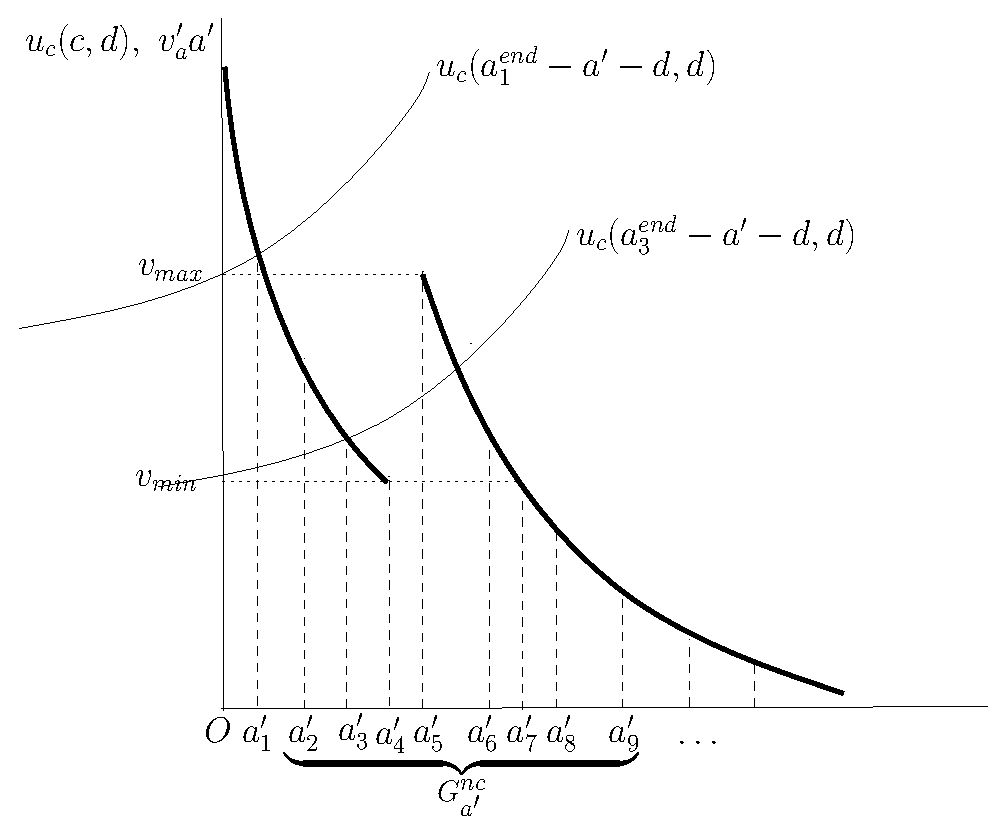
\includegraphics[scale=0.45]{Figure1_Appendix.eps} }
\end{center}
\end{figure}

Figure \ref{fig:egm} plots the right and left hand sides of equation EE as a
function of $a'$ for a given value of $d,$ The left hand side is plotted
for two possible values of initial assets $a.$ For given $a,$ the
intersection of the two curves is a candidate solution for the saving
correspondence $a'(a|d)$ \emph{conditional} on the given value of $d.$
The contribution of \citeasnoun{Fella_egm11} concerns how to solve for
this ``conditional'' saving correspondence $a'(a|d)$.

In the standard approach, one fixes values for the endogenous state
variable $a$ at the beginning of the period and solves the Euler
equation forward for the associated values of end-of-period wealth
$a'$. \possessivecite{Carroll-eclet06} endogenous grid method (EGM),
instead, fixes an ordered grid $G_{a'}=\{a'_{1},a'_{2},\ldots, a'_{m}\}$
for \emph{end-of-period} assets $a'$ and solve for the value of
\emph{initial wealth} $a^{end}_{i}$ that satisfies EE for each
$a'_{i}\in G_{a'}.$ for each $a'_{i}\in G_{a'}.$\footnote{In terms of
  Figure  \ref{fig:egm}, at the grid point $a_{1}',$ for example, the EGM
  solves for the value of initial assets $a_{1}^{end}$ associated with
  the unique element of the family of upward sloping curves, indexed by
  initial wealth $a,$ that intersects $v_{a}'(a')$ at point $a'_{1}.$}
This approach is substantially faster as the Euler equation is often
linear in consumption, hence in $a$, but non-linear (and in our case not
even continuous) in $a'$.

Since, given the non-concavity of the problem, a local maximum is not
necessary a global one, the algorithm modifies the standard EGM in the
following way. First, it partitions the set of grid points for future
assets $G_{a'}$ into a \emph{non-concave region} $G_{a'}^{nc}$ in which
the Euler equation is not sufficient for a global maximum for $a'$ and
its set complement.  In terms of Figure   \ref{fig:egm}, given the grid
$G_{a'}$ and the derivative of the continuation value $v_{a}(a')$ it
determines the \emph{non-concave region} $G_{a'}^{nc}$ as the set of
grid points for which $v'_{a}(a')\in(v_{min},v_{max}).$\footnote{In
Figure \ref{fig:egm}, $G_{a'}^{nc}=\{a'_{2},\ldots,a'_{6}\}.$ }
Secondly, for all $a_{i}'$ in the non-concave region, the algorithm
supplements EGM with a global maximization step.

More formally, given $G_{a'},$ $v'_{a}(a')$ for $a'\in G_{a'}$ and $d$
\begin{enumerate}
\item Determine the non-concave region $G^{nc}_{a'}.$ Initialize the
  counters $i=1$ and $l=1$
\item Solve EE for $a^{end}_{i}$ given $a'_{i}$ using EGM.
\item If $a'_{i}\in G^{nc}_{a'}$ then
  \begin{itemize}
  \item find the maximizer of the discretized maximand for
    $a=a^{end}_{i};$ i.e. solve for
    \[
    a'_{g}=\arg \max _{a'\in G_{a'}^{nc}}u(a^{end}_{i}-a'-d,d)+v'(a').
    \]
  \item if $a'_{g}\neq a'_{i},$ $a'_{i}$ is not a global maximum. Move
    to the next grid point---$i=i+1$---and go to 2.
  \end{itemize}
\item Store the solution pair $(a^{end}_{i},a'_{i})$ as
  $(a^{end}_{i_{l}},a'_{i_{l}})=(a^{end}_{i},a'_{i}).$ As long as $a'$
  is not the last grid point, set $i=i+1, l=l+1$ and go to 2.
\item Having solved for the conditional saving correspondence
  $\{a^{end}_{i_{l}},a'_{i_{l}}\}$ on the endogenous collocation points
  $\{a^{end}_{i_{l}}\}$ solve for the conditional value function given
  $d$
\[
v_{i_{l}}=u(a_{il}^{end}-a'_{il}- d,d)+v'(a')
\]
\item Evaluate interpolating functions through $(a_{il}^{end},a'_{il})$
  and $(a_{il}^{end},v_{il})$ at $a\in G_{a'}$ to obtain the conditional
  policy and value functions $a'(a|d)$ and $v(a|d)$ on the original grid
  $ G_{a'}.$
\item Maximize $v(a|d)$ over $d$ to obtain $d(a)$ and $v(a)$.
  \end{enumerate}

  In a longer (possibly infinite) horizon case, having obtained $v(a)$
  one would compute its partial derivative $v_{a}(a)$ and would work
  backwards.

  \citeasnoun{Fella_egm11} compares the accuracy and speed of the method to that of discretized value function iteration (VFI)---the most
  commonly chosen algorithm for non-concave, non-differentiable problems---using a saving problem with a discrete durable and a continuous
  non-durable choice. The discrete non-durable choice can take seven values, which implies a number of potential discontinuities larger
  than in the current model. He finds that the modified EGM algorithm has an accuracy, measured by the average Euler error (in base 10 log
  points) over a simulated history, in excess of -5 already with only 200 grid points for the continuous wealth variable. This is more than
  twice the accuracy of VFI\footnote{The average Euler error, rather than the supremum of the Euler errors, is the sensible accuracy
    measure in a model with discontinuities in the policy function, since, no matter how large the number of grid points, the
    probability of interpolating across a discontinuity goes to one as the length of a history increases. The Euler error when
    interpolating across the discontinuity is determined by the size of the jump in the function. } for the same number of grid
  points.\footnote{In fact, the modified EGM with 200 grid points is still two orders of magnitudes more accurate, and 70 times faster,
    than VFI with 1000 grid points.}

\section{Appendix: College subsidy}
\label{sec:college-subsidy}
The main policy focus of our analysis has been the effect of high school subsidization. Such focus naturally relates to the existing literature---reviewed in \citeasnoun{Lochner_hbkee11}---on the effects of schooling on crime. In this literature a motivation for early intervention is that the majority of property crime is committed by people with relatively low education, and high school graduation has been proven effective in reducing crime.

In this appendix, instead, we analyze the effects of a policy that subsidizes college completion. In particular, we consider a transfer paid to all people who enroll and complete college.
%Only a subset of all high school graduates pursue a college education and therefore the scope of this policy is smaller and one should acknowledge that, from the government point of view, this policy might be harder to justify as a pure anti-crime measure, as it would be targeted to those relatively richer people who tend to go to college.
For comparability with the other policy experiments in the main body of the paper, we consider a college subsidy that achieves the same general equilibrium crime reduction as the high school subsidy equal to 8.8\% of average earnings studied in the paper. The size of the college subsidy that achieves the targeted victimization rate of 5.2\% is about 15.3\% of average earnings.

Table \ref{tab: coll-exp} reports the effects (relative to the benchmark) of the college subsidy in both partial and general equilibrium. In general equilibrium the policy costs as much as the high school subsidy policy, but it induces a somewhat smaller welfare gain. Intuitively a college subsidy provides less insurance against ex ante uncertainty, relative to the high school subsidy, as it primarily affects high ability individuals marginal to the college choice.

\begin{table}[h]
       %\footnotesize
       \centering
       \hspace*{-.5cm}\caption{College subsidy experiments. Subsidy as \% of average labor income.  }
       \hspace*{-.5cm}
       \begin{tabular}{lccc}
        \noalign{\medskip}
        \toprule
                    &  Benchmark & COL Subsidy PE & COL Subsidy GE      \\
        \midrule
                                 &  (1)  &   (2) &   (3)         \\
        COL subsidy              &  -    & 15.3  & 15.3          \\
Prison sentence (months)         & 19    & 19    & 19            \\
Crime victimization (\%)         & 5.6   & 5.9   & 5.2           \\
Arrest rate L (\unichar{8241}) & 5.9   & 7.1   & 5.5             \\
Arrest rate H (\unichar{8241}) & 2.7   & 3.4   & 2.7             \\
L share of criminals (\%)      & 48    & 51.5  & 47              \\
                   Output        & 100.0 & -     & 101.6         \\
         Agg. Consumption        & 100.0 & -     & 102.1         \\
                  Welfare        & 100.0 & 106.3 & 103.1         \\
Prison expenditure$^\dagger$     & 0.30  & 0.31  & 0.28          \\
Subsidy + prison exp.$^\dagger$  & 0.30  & 0.88  & 0.51          \\
           Price L             & 100.0 & -     & 102.4           \\
           Price H             & 100.0 & -	 & 102.3             \\
           Price C	             & 100.0 & -	 & 97.9          \\
       \bottomrule
       \multicolumn{4}{l}{$^\dagger$ As a share of aggregate consumption in the benchmark.}
       \end{tabular}%
       \label{tab: coll-exp}
\end{table}%

To understand what drives the general equilibrium response, it is instructive to consider what the effect would be in partial equilibrium. The policy actually \emph{increases} the crime rate by almost 0.3 percentage points in partial equilibrium as it induces a very large rise in college completion. The size of the subsidy, together with the relatively low cost of college attendance in 1980, implies that college education becomes not only free at the point of entry, but is associated to a non-trivial monetary transfer. Such large shift in college completion, at constant prices, increases income inequality and the average return from crime. In contrast, the high school subsidy actually \emph{reduces} the crime rate by a similar amount already in partial equilibrium. Therefore, all of the crime reduction effects of the college subsidy are due to general equilibrium effects. These are even larger than in the case of the high school subsidy, as the college subsidy substantially increases the human capital price not only for high school dropouts, but also for high school graduates. The resulting increase in earnings among the lowest two education groups raises the opportunity cost of engaging in crime for those agents who are most likely to commit crime. The difference between partial and general equilibrium is stark and highlights the importance of general equilibrium adjustments, which would  be the only anti-crime justification for implementing such a policy.

Finally, one word of warning is necessary when assessing these results on the effects of a universal college subsidy. The direct costs of attending college have been steadily increasing over time, and continue to do so. As we mentioned above, a universal college subsidy of 15.3\% (the one considered in this experiment) would have resulted, in 1980, in free college at the point of entry plus a yearly handout equal to roughly half the college cost. The same proportional subsidy in 2000, when college tuitions were more than double those in 1980, would instead have covered only between half and two thirds of the direct cost of college.


\bibliographystyle{econometrica}
\begin{thebibliography}{xx}

\harvarditem[Barillas and Fern\'{a}ndez-Villaverde]{Barillas and Fern\'{a}ndez-Villaverde}{2007}{BarillasVillaverde_jedc07}
\textsc{Barillas, F.,  {\small and} J.~Fern\'{a}ndez-Villaverde}  (2007): ``A
  Generalization of the Endogenous Grid Method,'' \emph{Journal of Economic
  Dynamics and Control}, 31, 2698--2712.

\harvarditem[Carroll]{Carroll}{2006}{Carroll-eclet06}
\textsc{Carroll, C.~D.}  (2006): ``The Method of Endogenous Gridpoints for
  Solving Dynamic Stochastic Optimization Problems,'' \emph{Economics Letters},
  91, 312--320.

\harvarditem[Clausen and Strub]{Clausen and Strub}{2012}{clausenstrub_wp10}
\textsc{Clausen, A.,  {\small and} C.~Strub}  (2012): ``Envelope Theorems for
  Non-Smooth and Non-Concave Optimization,'' Mimeo, University of Pennsylvania.

\harvarditem[Fella]{Fella}{2014}{Fella_egm11}
\textsc{Fella, G.}  (2014): ``A Generalized Endogenous Grid Method for
  Non-Smooth and Non-Concave Problems,'' \emph{Review of Economic Dynamics},
17, 329-344.

\harvarditem[Lochner]{Lochner}{2011}{Lochner_hbkee11}
\textsc{Lochner, L.}  (2011): ``Chapter 2 - Nonproduction Benefits of Education:
  Crime, Health, and Good Citizenship,'' in \emph{Handbook of The Economics of
  Education}, ed. by E.~A. Hanushek, S.~Machin,  {\small and} L.~Woessmann,
  vol.~4 of \emph{Handbook of the Economics of Education}, pp. 183 -- 282.
  Elsevier.

\end{thebibliography}

\end{document}
